\documentclass[10pt,a4paper]{article}
\usepackage[english,brazil]{babel}
\usepackage[utf8]{inputenc}
\usepackage{amsmath}
\usepackage{amssymb}
\usepackage{graphicx}
\newtheorem{definition}{Definição}[section]
\graphicspath{{figuraspdf/}}


\begin{document}

\section{Estudo da bibliografia}

Este arquivo serve para fazer apontamentos acerca da bibliografia indicada/pesquisada.

\subsection{Estudo do artigo  \cite{lee94}}.

A matriz de espalhamento complexa {\bf S} é definida por

$$
{\bf s} = \left[
\begin{array}{cc}
	S_{hh}   & S_{hv}   \\
	S_{vh}   & S_{vv}   \\
\end{array}
\right].
$$

Por facilidade usaremos o fato de ser um {\it reciprocal medium}, isto é, $S_{hv}=S_{vh}$
$$
{\bf s} = \left[
\begin{array}{c}
	S_{vv}      \\
	S_{vh}     \\
	S_{hh}      \\
\end{array}
\right].
$$

De acordo com \cite{goodman1963} a distribuíção gaussiana complexa multivariada pode modelar adequadamente o comportamento estatístico de $\bf S$. Isto é chamado de {\it single-look PolSar data representation} e podemos definir o vetor de espalhamento por ${\bf s}=[S_1,S_2,\dots,S_p]^T$. 

A função densidade de probabilidade ({\bf pdf}) da distribuição gaussiana complexa $p-$variada é dada por
\begin{equation}\label{sec1eqn2}
\begin{array}{ccc}
	p({\bf s})&=&\frac{1}{\pi^p|\Sigma_{{\bf s}}|}\exp(-\bar{{\bf s}}^{T}\Sigma_{{\bf s}}^{-1}{\bf s})  \\
\end{array}
\end{equation}

Sendo a matriz de covariância definida por:
\begin{equation}\label{sec1eqn2}
	{\bf \Sigma_{{\bf s}}} = E[{\bf s}{\bf s}^H] = \left[
\begin{array}{cccc}
	E({\bf s_1}{\bf s_1}^H)  & E({\bf s_1}{\bf s_2}^H) &\hdots & E({\bf s_1}{\bf s_p}^H) \\
	E({\bf s_2}{\bf s_1}^H)  & E({\bf s_2}{\bf s_2}^H) &\hdots &E({\bf s_2}{\bf s_p}^H)\\
        \vdots&\vdots &\ddots &\vdots\\
	E({\bf s_p}{\bf s_1}^H)  & E({\bf s_p}{\bf s_2}^H) &\hdots &E({\bf s_p}{\bf s_p}^H)\\
\end{array}
\right].
\end{equation}

onde $E(\cdot)$ e $(\cdot)^H$ denotam o valor esperado e o conjugado transposto.

Dados polarimétricos são usualmente sujeitados a um processo {\it multilook} com o intuito de melhorar a razão {\it signal-to-noise}. Para esse fim, matrizes positivas definidas hermitianas são obtidas computando a médias de $L$ {\it looks} independentes de uma mesma cena. Isto resulta na matriz de covariância {\bf Z} dada por:

\begin{equation}\label{sec1eqn3}
\begin{array}{ccc}
	{\bf Z}&=&\frac{1}{n}\displaystyle{\sum_{i=1}^{L} {\bf s_i}{\bf s_i}^H} . \\
\end{array}
\end{equation}

\subsection{Estudo do artigo  \cite{goodman1963}}


A variável randômica gaussiana complexa ${\bf Z=X+iY}$ é uma variável randômica complexa cuja parte imaginária e complexa são distribuída de forma Gaussiana.  E uma variável randômica gaussiana complexa $p-$variada $\xi^{'}=(Z_1,Z_2,\dots,Z_p)$ é uma $p-$upla  de variáveis randômica gaussiana complexas tal que o vetor de partes imaginárias e reais é $\eta^{'}=(X_1,Y_1,\dots,X_p,Y_p)$.

A matriz de covariância definida positiva $2p\times 2p$ será:
$$
{\bf \Sigma_{\eta}} = \left[
\begin{array}{cc}
	E(X_jX_k)  & E(X_jY_k)  \\
	E(Y_jX_k)  & E(Y_jY_k)  \\
\end{array}
\right].
$$
Tal que
$$
{\bf \Sigma_{\eta}} = \left[
\begin{array}{cc}
	E(X_jX_k)  & E(X_jY_k)  \\
	E(Y_jX_k)  & E(Y_jY_k)  \\
\end{array}
\right]= \left\{
\begin{array}{cc}
	\frac{1}{2}\left[
\begin{array}{cc}
	 1 & 0  \\
	 0 & 1  \\
\end{array}
	\right]\sigma^{2}_{k}  & \mbox{se}\quad j=k, \\
	& \\
	\frac{1}{2}\left[
\begin{array}{cc}
	\alpha_{ik} & -\beta_{jk}  \\
	 \beta_{jk} & \alpha_{ik}  \\
\end{array}
	\right]\sigma_j\sigma_k  & \mbox{se}\quad j\neq k.   \\
\end{array}
\right.
$$

Onde $E(\cdot)$ denota o operador de valor esperado(esperança).

Podemos usar a matriz de covariância hermitiana complexa definida positiva usando a $\xi$ variável randômica gaussiana complexa de dimensão $p\times p$

$$\Sigma_{\xi}=E(\xi\bar{\xi}^{T})=||E(Z_j\bar{Z}_k)||=||\sigma_{jk}||$$

onde

$$
\sigma_{jk} = \left\{
\begin{array}{cc}
	\sigma_k^2                                & \mbox{se}\quad j=k,  \\
	(\alpha_{jk}+i\beta_{jk})\sigma_j\sigma_k & \mbox{se}\quad j\neq k. \\
\end{array}
\right.
$$

A função densidade de probabilidade ({\bf pdf}) da distribuição gaussiana complexa $p-$variada é dada por
\begin{equation}\label{sec2eqn1}
\begin{array}{ccc}
	p(\xi)&=&\frac{1}{\pi^p|\Sigma_{\xi}|}\exp(-\bar{\xi}^{T}\Sigma_{\xi}^{-1}\xi)  \\
\end{array}
\end{equation}


{\bf Exemplo 1 -} Seja a distribuição gaussian complexa univariada $(p=1)$. Sendo $\xi^{T}=z_1=x_1+iy_1$. E a "matriz" de covariância $\Sigma_{\xi}=\sigma_{1}^{2}$ com determinante $|\Sigma_{\xi}|=\sigma_{1}^{2}$ e  "matriz inversa" $\Sigma_{\xi}^{-1}=\frac{1}{\sigma_{1}^{2}}$, Assim,

\begin{equation}\label{sec2eqn2}
\begin{array}{ccc}
	\bar{\xi}^{T}\Sigma_{\xi}^{-1}\xi&=&(x_i-iy_1)\frac{1}{\sigma_1^2}(x_1+iy_1)  \\
	\bar{\xi}^{T}\Sigma_{\xi}^{-1}\xi&=&(x_i-iy_1)(x_1+iy_1)\frac{1}{\sigma_1^2}  \\
	\bar{\xi}^{T}\Sigma_{\xi}^{-1}\xi&=&\frac{x_1^2+y_1^2}{\sigma_1^2}  \\
\end{array}
\end{equation}


\begin{equation}\label{sec2eqn3}
\begin{array}{ccc}
	p(\xi)&=&\frac{1}{\pi\Sigma_{\xi}^{2}}\exp\left(-\frac{x_1^2+y_1^2}{\sigma_1^2}\right)  \\
\end{array}
\end{equation}

{\bf Exemplo 2 -} Seja a distribuição gaussian complexa bivariada $(p=2)$. Sendo $\xi^{T}=(z_1, z_2)=(x_1 + iy_1, x_2 + iy_2)^{T}$. E a matriz de covariância 

$$
\Sigma_{\xi} = \left[
\begin{array}{cc}
	\sigma_1^2                                &  (\alpha_{12}+i\beta_{12})\sigma_1\sigma_2  \\
	(\alpha_{12}-i\beta_{12})\sigma_j\sigma_k & \sigma_2^2 \\
\end{array}
\right].
$$
com determinante $|\Sigma_{\xi}|=(1 - \sigma_{12}^{2}- \beta_{12}^2)\sigma_{1}^2\sigma_{2}^2$ e  matriz inversa 
$$
\Sigma_{\xi}^{-1} =\frac{1}{(1 - \sigma_{12}^{2}- \beta_{12}^2)\sigma_{1}^2\sigma_{2}^2} \left[
\begin{array}{cc}
	\sigma_2^2                                &  -(\alpha_{12}+i\beta_{12})\sigma_1\sigma_2  \\
	-(\alpha_{12}-i\beta_{12})\sigma_j\sigma_k & \sigma_1^2 \\
\end{array}
\right].
$$
\begin{equation}\label{sec2eqn4}
\begin{array}{ccc}
	\bar{\xi}^{T}\Sigma_{\xi}^{-1}\xi&=&[z_1,z_2]^{H}\Sigma_{\xi}^{-1}
	\left[
\begin{array}{c}
	z_1  \\
	z_2 \\
\end{array}\right]\\
\end{array}
\end{equation}
\begin{equation}\label{sec2eqn5}
\begin{array}{ccc}
	\bar{\xi}^{T}\Sigma_{\xi}^{-1}\xi&=&[z_1,z_2]^{H}\frac{1}{(1 - \sigma_{12}^{2}- \beta_{12}^2)\sigma_{1}^2\sigma_{2}^2} \left[
\begin{array}{cc}
	\sigma_2^2                                &  -(\alpha_{12}+i\beta_{12})\sigma_1\sigma_2  \\
	-(\alpha_{12}-i\beta_{12})\sigma_1\sigma_2 & \sigma_1^2 \\
\end{array}
\right]
	\left[
\begin{array}{c}
	z_1  \\
	z_2 \\
\end{array}\right]\\
\end{array}
\end{equation}

\begin{equation}\label{sec2eqn6}
\begin{array}{ccc}
	\bar{\xi}^{T}\Sigma_{\xi}^{-1}\xi&=&\frac{1}{(1 - \sigma_{12}^{2}- \beta_{12}^2)\sigma_{1}^2\sigma_{2}^2} [z_1,z_2]^{H}\left[
\begin{array}{cc}
	\sigma_2^2                                &  -(\alpha_{12}+i\beta_{12})\sigma_1\sigma_2  \\
	-(\alpha_{12}-i\beta_{12})\sigma_1\sigma_2 & \sigma_1^2 \\
\end{array}
\right]
	\left[
\begin{array}{c}
	z_1  \\
	z_2 \\
\end{array}\right]\\
\end{array}
\end{equation}

\begin{equation}\label{sec2eqn7}
\begin{array}{ccc}
	\bar{\xi}^{T}\Sigma_{\xi}^{-1}\xi&=&\frac{1}{(1 - \sigma_{12}^{2}- \beta_{12}^2)\sigma_{1}^2\sigma_{2}^2} [z_1,z_2]^{H}\left[
\begin{array}{cc}
	\sigma_2^2z_1-(\alpha_{12}+i\beta_{12})\sigma_1\sigma_2z_2  \\
	-(\alpha_{12}-i\beta_{12})\sigma_1\sigma_2z_1+\sigma_1^2z_2 \\
\end{array}
\right]
\end{array}
\end{equation}

\begin{equation}\label{sec2eqn8}
\begin{array}{ccc}
	\bar{\xi}^{T}\Sigma_{\xi}^{-1}\xi&=&\frac{1}{(1 - \sigma_{12}^{2}- \beta_{12}^2)\sigma_{1}^2\sigma_{2}^2}\left(
\begin{array}{c}
	\sigma_2^2\bar{z_1}z_1-(\alpha_{12}+i\beta_{12})\sigma_1\sigma_2\bar{z_1}z_2 
	-(\alpha_{12}-i\beta_{12})\sigma_1\sigma_2\bar{z_2}z_1+\sigma_1^2\bar{z_2}z_2 \\
\end{array}
	\right)
\end{array}
\end{equation}

\begin{equation}\label{sec2eqn9}
\begin{array}{ccc}
	\bar{\xi}^{T}\Sigma_{\xi}^{-1}\xi&=&\frac{1}{(1 - \sigma_{12}^{2}- \beta_{12}^2)\sigma_{1}^2\sigma_{2}^2}\left(
\begin{array}{c}
	\sigma_2^2|z_1|^2+\sigma_1^2|z_2|^2-2\alpha_{12}\sigma_1\sigma_2\bar{z_1}z_2 \\
\end{array}
	\right)
\end{array}
\end{equation}

\begin{equation}\label{sec2eqn10}
\begin{array}{ccc}
	\bar{\xi}^{T}\Sigma_{\xi}^{-1}\xi&=&\frac{\sigma_2^2|z_1|^2+\sigma_1^2|z_2|^2-2\alpha_{12}\sigma_1\sigma_2\bar{z_1}z_2}{(1 - \sigma_{12}^{2}- \beta_{12}^2)\sigma_{1}^2\sigma_{2}^2}
\end{array}
\end{equation}

Assim, a função densidade de probabilidade ({\bf pdf}) 

\begin{equation}\label{sec2eqn11}
\begin{array}{ccc}
	p(\xi)&=&\frac{1}{\pi^2(1 - \sigma_{12}^{2}- \beta_{12}^2)\sigma_{1}^2\sigma_{2}^2}\exp\left(-\frac{\sigma_2^2|z_1|^2+\sigma_1^2|z_2|^2-2\alpha_{12}\sigma_1\sigma_2\bar{z_1}z_2}{(1 - \sigma_{12}^{2}- \beta_{12}^2)\sigma_{1}^2\sigma_{2}^2}
\right)  \\
\end{array}
\end{equation}

{\bf Distribuição complexa de Wishart}

A distribuição complexa de Wishart descrita no artigo \cite{goodman1963}, define agora uma amostra de  $n$ vetores com valores complexos $\xi_1,\xi_2,\dots,\xi_n$ então a matriz hermitiana de covariância é 

\begin{equation}\label{sec2eqn12}
\begin{array}{ccc}
	\hat{\Sigma}_{\xi}&=&\frac{1}{n}\displaystyle{\sum_{j=1}^{n}\xi_j\bar{\xi}_{j}^{T}} . \\
\end{array}
\end{equation}

A matriz $\hat{\Sigma}_{\xi}$ é uma "maximum likelihood" para $\Sigma_{\xi}$ sendo uma estatística suficiente para a matriz hermitiana de covariância.

Considerando $A=||A_{jkR}+iA{jkI}||=n\hat{\Sigma}_{\xi}$ chamaremos a matriz $A$ de distribuição complexa de Wishart. A função densidade de probabilidade de $A$ é


\begin{equation}\label{sec2eqn13}
\begin{array}{ccc}
	p_W(A)&=&\frac{|A|^{n-p}}{I(\Sigma_{\xi})} \exp(-tr(\Sigma_{\xi}^{-1}A)), \\
\end{array}
\end{equation}
onde
\begin{equation}\label{sec2eqn14}
\begin{array}{ccc}
	I(\Sigma_{\xi})&=&\pi^{\frac{1}{2}p(p-1)}\Gamma(n)\dots\Gamma(n-p+1)|\Sigma_{\xi}|^n, \\
\end{array}
\end{equation}
sendo $\Gamma(\cdot)$ a função Gamma.

\subsection{Estudo do artigo  \cite{salicru_pardo_1994}}

Definição importante  

\begin{definition}{Divergência ($h,\phi$).}
	Sejam as variáveis aleatórias $X$ e $Y$ com mesmo suporte $S$  e $p.d.f$ respectivamente $f_{X}(x|\theta_1)$ e $f_{Y}(x|\theta_2)$. Sejam ainda $\phi:(0,\infty)\rightarrow \mathbb{R}_+$ uma função convexa e diferenciável, e $h$ uma função crescente tal que $h(0)=0$ então a divergência ($h,\phi$) é definida como
\begin{equation}\label{sec3eqn1}
\begin{array}{ccc}
	d_{\phi}^{h}(X||Y)&=&\displaystyle{h\left[\int_{x\in S(x)} f_{Y}(x|\theta_2)\phi\left(\frac{f_{X}(x|\theta_1)}{f_{Y}(x|\theta_2)}\right)dx \right]}. \\
\end{array}
\end{equation}
\end{definition}

Definindo que divergência é uma maneira de medir as diferenças entre duas distribuições. A seguir descreveremos um exemplo para ilustrar a definição.

Para começar a entender os resultados do artigo \cite{salicru_pardo_1994} é descrito abaixo o exemplo 1 sobre medida craniana de rãs:

Sendo $(x_1)$ o comprimento craniano e $(x_2)$ a amplitude craniana, uma amostra de $n=35$ rãs femeas maduras conduziu a seguinte estatística:

$$
{\bf x_1} = \left[
\begin{array}{c}
	22.860   \\
	24.397   \\
\end{array}
\right]
{\bf S_1} = \left[
\begin{array}{cc}
	 17.178  & 19.710   \\
         19.710  & 23.710   \\
\end{array}
\right].
$$

e similar medidas para uma amostra $m=14$ rãs machos, 

$$
{\bf x_2} = \left[
\begin{array}{c}
	21.821  \\
	22.843   \\
\end{array}
\right]
{\bf S_2} = \left[
\begin{array}{cc}
	 17.159  & 17.731   \\
         17.731  & 19.273   \\
\end{array}
\right].
$$

onde ${\bf S_1}$ e ${\bf S_2}$ são estimadores de máxima varossimilhança da matriz de covariância.

Para auxiliar foi criado dois programas em matlab chamados "salicruex1a.m" e "salicru1ex1b.m" armazenado em (meu micro): $$"/home/aborba/MEGAsync/mack/alejandro/gitufalmackbackup/doclatex/"$$


\begin{description}
\item[(a)] Sendo:
$$
		{\bf S}=\frac{n{\bf S_1}+m{\bf S_2}}{n+m} = \left[
\begin{array}{cc}
	 17.173  & 19.145   \\
         19.145  & 22.442   \\
\end{array}
\right].
$$
tal que sua matriz inversa é:
$$
		{\bf S^{-1}} = \left[
\begin{array}{cc}
	 1.18958  & -1.01482   \\
        -1.01482.  & 0.91028   \\
\end{array}
\right].
$$

		A expressão $(r,s)$-divergência obtida de $(h,\phi)$-divergência sobre certas condições pode ser escrita:
\begin{equation}\label{sec3eqn2}
\begin{array}{ccl}
	D_r^s((\mu_1,\Sigma_1),(\mu_2,\Sigma_2))&=&\frac{1}{(s-1)}\left[\exp\left(\frac{r(s-1)}{2}(\mu_1-\mu_2)^{T}[r\Sigma_2+(1-r)\Sigma_1]^{-1}(\mu_1-\mu_2) \right)\right. \\
	&\cdot&\left.\frac{|r\Sigma_2+(1-r)\Sigma_1|^{\frac{(1-s)}{2(r-1)}}}{|\Sigma_1|^{\frac{s-1}{2}}|\Sigma_2|^{\frac{(1-s)r}{2(r-1)}}}-1\right]  \\
\end{array}
\end{equation}

Assim calculando
\begin{equation}\label{sec3eqn3}
\begin{array}{ccc}
	T_4&=&\frac{2nm}{r(n+m)}D_r^s(({\bf x_1}, {\bf S}),({\bf x_2}, {\bf S})) \\
	T_4&=&40(0.052663) \\
	T_4&=&2.10653
\end{array}
\end{equation}
\item[(b)] Será usado o corolário $2b$ do artigo \cite{salicru_pardo_1994} assim a estatística que vamos calcular será:

\begin{equation}\label{sec3eqn4}
\begin{array}{ccc}
	T_3&=&\frac{2nm}{r(n+m)}D_r^s(({\bf x_1}, {\bf S_1}),({\bf x_2}, {\bf S_2})) \\
	T_3&=&4.76047
\end{array}
\end{equation}

Tendo um valor diferente do artigo, investigando onde pode estar a discrepância encontramos o seguinte valor para, 

\begin{equation}\label{sec3eqn5}
\begin{array}{ccc}
	({\bf x_1}-{\bf x_2})^T [r{\bf S_2+(1-r){\bf S_1}}]^{-1}({\bf x_1}-{\bf x_2})&=& 0.22724\\
\end{array}
\end{equation}

enquanto o artigo encontrou $0.06970$ para o mesmo passo, até o momento não sei explicar a diferença.

\end{description}


\subsection{Estudo do artigo  \cite{anfinsen2009}}

O instrumento SAR totalmente polarimétrico transmite pulsos de microondas polarizados ortogonalmente e mede componentes ortogonais do sinal recebido. Para cada pixel a medida resulta em uma matriz de coeficientes de espalhamento. Esses coeficientes são números complexos que descrevem a transformação do campo eletromagnético trasmitido para o campo eletromagnético recebido para todas as combinações de transmitidas e recebidas polarizações.

A transformação pode ser representada como

\begin{equation}\label{sec4eqn1}
 \left[
\begin{array}{c}
	E_{h}^{r}   \\
	E_{v}^{r}    \\
\end{array}
\right]
 = \frac{e^{jkr}}{r}\left[
\begin{array}{cc}
	S_{hh}   & S_{hv}   \\
	S_{vh}   & S_{vv}   \\
\end{array}
\right]
 \left[
\begin{array}{c}
	E_{h}^{t}   \\
	E_{v}^{t}    \\
\end{array}
\right]
\end{equation}

Onde $k$ denota o número de onda e $r$ é a distância entre o radar e o alvo. No campo eletromagnético com componentes $E_{i}^{j}$ os índices subscritos denotados polarização horizontal $h$ ou vertical $v$ enquanto os índices sobrescritos indicam a onda recebida $r$ ou transmitida $t$.    


A matrix de espalhamento pode ser reduzida ao seguintes vetores:

\begin{equation}\label{sec4eqn2}
{\bf s} = \left[
\begin{array}{c}
	S_{hh}      \\
	\frac{S_{hv}+S_{vh}}{\sqrt{2}}     \\
	S_{vv}      \\
\end{array}
\right].
{\bf k} =\frac{1}{\sqrt{2}} \left[
\begin{array}{c}
	S_{hh} + S_{vv}      \\
	S_{hh} - S_{vv}      \\
	S_{hv} + S_{vh}      \\
\end{array}
\right].
\end{equation}

%De acordo com \cite{goodman1963} a distribuíção gaussiana complexa multivariada pode modelar adequadamente o comportamento estatístico de $\bf S$. Isto é chamado de {\it single-look PolSar data representation} e podemos definir o vetor de espalhamento por ${\bf s}=[S_1,S_2,\dots,S_p]^T$. 

%A função densidade de probabilidade ({\bf pdf}) da distribuição gaussiana complexa $p-$variada é dada por
%\begin{equation}\label{sec1eqn2}
%\begin{array}{ccc}
%	p({\bf s})&=&\frac{1}{\pi^p|\Sigma_{{\bf s}}|}\exp(-\bar{{\bf s}}^{T}\Sigma_{{\bf s}}^{-1}{\bf s})  \\
%\end{array}
%\end{equation}

%Sendo a matriz de covariância definida por:
%\begin{equation}\label{sec1eqn2}
%	{\bf \Sigma_{{\bf s}}} = E[{\bf s}{\bf s}^H] \left[
%\begin{array}{cccc}
%	E({\bf s_1}{\bf s_1}^H)  & E({\bf s_1}{\bf s_2}^H) &\hdots & E({\bf s_1}{\bf s_p}^H) \\
%	E({\bf s_2}{\bf s_1}^H)  & E({\bf s_2}{\bf s_2}^H) &\hdots &E({\bf s_2}{\bf s_p}^H)\\
%        \vdots&\vdots &\ddots &\vdots\\
%	E({\bf s_p}{\bf s_1}^H)  & E({\bf s_p}{\bf s_2}^H) &\hdots &E({\bf s_p}{\bf s_p}^H)\\
%\end{array}
%\right].
%\end{equation}

%onde $E(\cdot)$ e $(\cdot)^H$ denotam o valor esperado e o conjugado transposto.

%Dados polarimétricos são usualmente sujeitados a um processo {\it multilook} com o intuito de melhorar a razão {\it signal-to-noise}. Para esse fim, matrizes positivas definidas hermitianas são obtidas computando a médias de $L$ {\it looks} independentes de uma mesma cena. Isto resulta na matriz de covariância {\bf Z} dada por:

%\begin{equation}\label{sec1eqn3}
%\begin{array}{ccc}
%	{\bf Z}&=&\frac{1}{n}\displaystyle{\sum_{i=1}^{L} {\bf s_i}{\bf s_i}^H} . \\
%\end{array}
%\end{equation}

\subsubsection{Modelos Gaussianos}


Podemos assumir que o vetor de espalhamento é uma distribuíção gaussiana complexa circular. A matriz {\bf S} e os vetores {\bf s} e {\bf k} são {\it Single-look complex} representação dos daos PolSAR. Dados PolSAR {\it Multilook} podem ser representados por
 
\begin{equation}\label{sec41eqn1}
\begin{array}{ccc}
	{\bf C_{\bf s}}&=&\frac{1}{L}\displaystyle{\sum_{i=1}^{L} {\bf s_i}{\bf s_i}^H} . \\
\end{array}
\begin{array}{ccc}
	{\bf C_{\bf k}}&=&\frac{1}{L}\displaystyle{\sum_{i=1}^{L} {\bf k_i}{\bf k_i}^H} . \\
\end{array}
\end{equation}

chamadas de matriz de covariância e matriz de coerência, sendo $L$ o número de {\it looks}. Por definição assumimos que {\bf s} ou {\bf k} é gaussiana multivariada e complexa circular e tem média zero. Será denotado $s\sim N_d^{\mathbb C}(\bf 0, \Sigma_{\bf s})$ onde $\bf 0$ é um vetor coluna de zeros, $d$ a dimensão de $\bf s$ a matriz de covariância de $\bf s$  

\begin{equation}\label{sec41eqn2}
	{\bf \Sigma_{{\bf s}}} = E[{\bf s}{\bf s}^H] =\left[
\begin{array}{cccc}
	E({\bf s_1}{\bf s_1}^H)  & E({\bf s_1}{\bf s_2}^H) &\hdots & E({\bf s_1}{\bf s_p}^H) \\
	E({\bf s_2}{\bf s_1}^H)  & E({\bf s_2}{\bf s_2}^H) &\hdots &E({\bf s_2}{\bf s_p}^H)\\
        \vdots&\vdots &\ddots &\vdots\\
	E({\bf s_p}{\bf s_1}^H)  & E({\bf s_p}{\bf s_2}^H) &\hdots &E({\bf s_p}{\bf s_p}^H)\\
\end{array}
\right].
\end{equation}

A função densidade de probabilidade $(pdf)$ de {\bf s} é 

\begin{equation}\label{sec41eqn3}
\begin{array}{ccc}
	p({\bf s},\Sigma_{\bf s})&=&\frac{1}{\pi^p|\Sigma_{{\bf s}}|}\exp(-{\bf s}^{H}\Sigma_{{\bf s}}^{-1}{\bf s})  \\
\end{array}
\end{equation}

Se $L\geq d$ e os {\bf $S_i$} (ou {\bf $k_i$}) e na equação (\ref{sec41eqn1}) são independentes, então ma matriz de covariância escalada pode ser definida como ${\bf Z}=L{\bf C_{\bf s}}$ (ou ${\bf Z}=L{\bf C_{\bf k}}$), de acordo com distribuição de Wishart complexa não singular \cite{goodman1963}

\begin{equation}\label{sec41eqn4}
\begin{array}{ccc}
	p_{{\bf Z}}({\bf Z};L,{\bf \Sigma})&=&\frac{|{\bf Z}|^{L-p}}{|{\bf \Sigma}|^{L}\Gamma_d(L)} \exp(-tr({\bf \Sigma}^{-1}{\bf Z})), \\
\end{array}
\end{equation}
onde $tr(\cdot)$ é o operador traço e ${\Sigma}=\frac{E[{\bf Z}]}{L}=E[{\bf C_{s}}]$. 

Vamos escrever ${\bf Z}\sim W_d^{\mathbb C}(L, {\bf \Sigma})$.

E ainda, A constante de normalização $\Gamma_d(L)$ é a função Gamma multivariada definida como 
\begin{equation}\label{sec41eqn5}
\begin{array}{ccc}
	\Gamma_d(L)&=&\pi^{\frac{1}{2}d(d-1)} \displaystyle{\prod_{i=0}^{d-1}\Gamma(L-i)} \\
\end{array}
\end{equation}
sendo $\Gamma(\cdot)$ a função Gamma.

Seja a distribuíção complexa Wishart (\ref{sec41eqn4}) vamos encontrar a derivada do logaritmo natural desta distribuição em relação ao número de {\it looks}.


\begin{equation}\label{sec41eqn6}
\begin{array}{ccc}
	\ln{\left(p_{{\bf Z}}({\bf Z};L,{\bf \Sigma})\right)}&=&\ln{\left(\frac{|{\bf Z}|^{L-p}}{|{\bf \Sigma}|^{L}\Gamma_d(L)} \exp(-tr({\bf \Sigma}^{-1}{\bf Z}))\right)}, \\
	\ln{\left(p_{{\bf Z}}({\bf Z};L,{\bf \Sigma})\right)}&=&\ln{\left(\frac{|{\bf Z}|^{L-p}}{|{\bf \Sigma}|^{L}\Gamma_d(L)}\right)}\ln{\left( \exp(-tr({\bf \Sigma}^{-1}{\bf Z}))\right)}, \\
	\ln{\left(p_{{\bf Z}}({\bf Z};L,{\bf \Sigma})\right)}&=&\ln{\left(|{\bf Z}|^{L-p}\right)} - \ln{\left(|{\bf \Sigma}|^{L}\Gamma_d(L)\right)}-tr({\bf \Sigma}^{-1}{\bf Z}), \\
	\ln{\left(p_{{\bf Z}}({\bf Z};L,{\bf \Sigma})\right)}&=&(L-p)\ln{\left(|{\bf Z}|\right)} - \ln{\left(|{\bf \Sigma}|^{L}\right)}-\ln{\left(\Gamma_d(L)\right)}-tr({\bf \Sigma}^{-1}{\bf Z}), \\
	\ln{\left(p_{{\bf Z}}({\bf Z};L,{\bf \Sigma})\right)}&=&L\ln{\left(|{\bf Z}|\right)}-p\ln{\left(|{\bf Z}|\right)} - L\ln{\left(|{\bf \Sigma}|\right)}-\ln{\left(\Gamma_d(L)\right)}-tr({\bf \Sigma}^{-1}{\bf Z}). \\
\end{array}
\end{equation}

Derivando a o logaritmo da distribuição em relação a $L$ teremos:
\begin{equation}\label{sec41eqn7}
\begin{array}{ccc}
	\frac{\partial}{\partial L}\left(\ln{\left(p_{{\bf Z}}({\bf Z};L,{\bf \Sigma})\right)}\right)&=&\frac{\partial}{\partial L}\left(L\ln{\left(|{\bf Z}|\right)}-p\ln{\left(|{\bf Z}|\right)} - L\ln{\left(|{\bf \Sigma}|\right)}-\ln{\left(\Gamma_d(L)\right)}-tr({\bf \Sigma}^{-1}{\bf Z})\right). \\
	\frac{\partial}{\partial L}\left(\ln{\left(p_{{\bf Z}}({\bf Z};L,{\bf \Sigma})\right)}\right)&=&\ln{\left(|{\bf Z}|\right)} - \ln{\left(|{\bf \Sigma}|\right)}-\frac{\partial}{\partial L}\left(\ln{\left(\Gamma_d(L)\right)}\right). \\
	\frac{\partial}{\partial L}\left(\ln{\left(p_{{\bf Z}}({\bf Z};L,{\bf \Sigma})\right)}\right)&=&\ln{\left(\frac{|{\bf Z}|}{|{\bf \Sigma}|}\right)} - \frac{\Gamma^{'}_d(L)}{\Gamma_d(L)}. \\
\end{array}
\end{equation}

isto é, 

\begin{equation}\label{sec41eqn8}
\begin{array}{ccc}
	\frac{\partial}{\partial L}\left(\ln{\left(p_{{\bf Z}}({\bf Z};L,{\bf \Sigma})\right)}\right)&=&\ln{\left(\frac{|{\bf Z}|}{|{\bf \Sigma}|}\right)} - \frac{\Gamma^{'}_d(L)}{\Gamma_d(L)}. \\
\end{array}
\end{equation}
\subsubsection{Coeficiente de estimador de variação}

 O exemplo da figura (\ref{sec41fig1}) mostra uma distribuíção gamma $g(\sigma, L)$ parametrizada com intensidade média $\sigma=0.0358$ e com múmeros de {\it looks} $L=\{8,10,12\}$.

\begin{equation}\label{sec41eqn6}
\begin{array}{ccc}
	p_{I}(I;\sigma,L)&=&\frac{1}{\Gamma(L)}\left(\frac{L}{\sigma}\right)^L \exp(-\frac{LI}{\sigma}), \\
\end{array}
\end{equation}
onde intensidade média $\sigma$ e número de {\it looks} $L$ são parametros desta distribuição gamma.

{\bf obs 1} - Programa {\it proanfinsen2009.r} armazenado no meu computador pessoal.

\begin{figure}[!h]
\centering
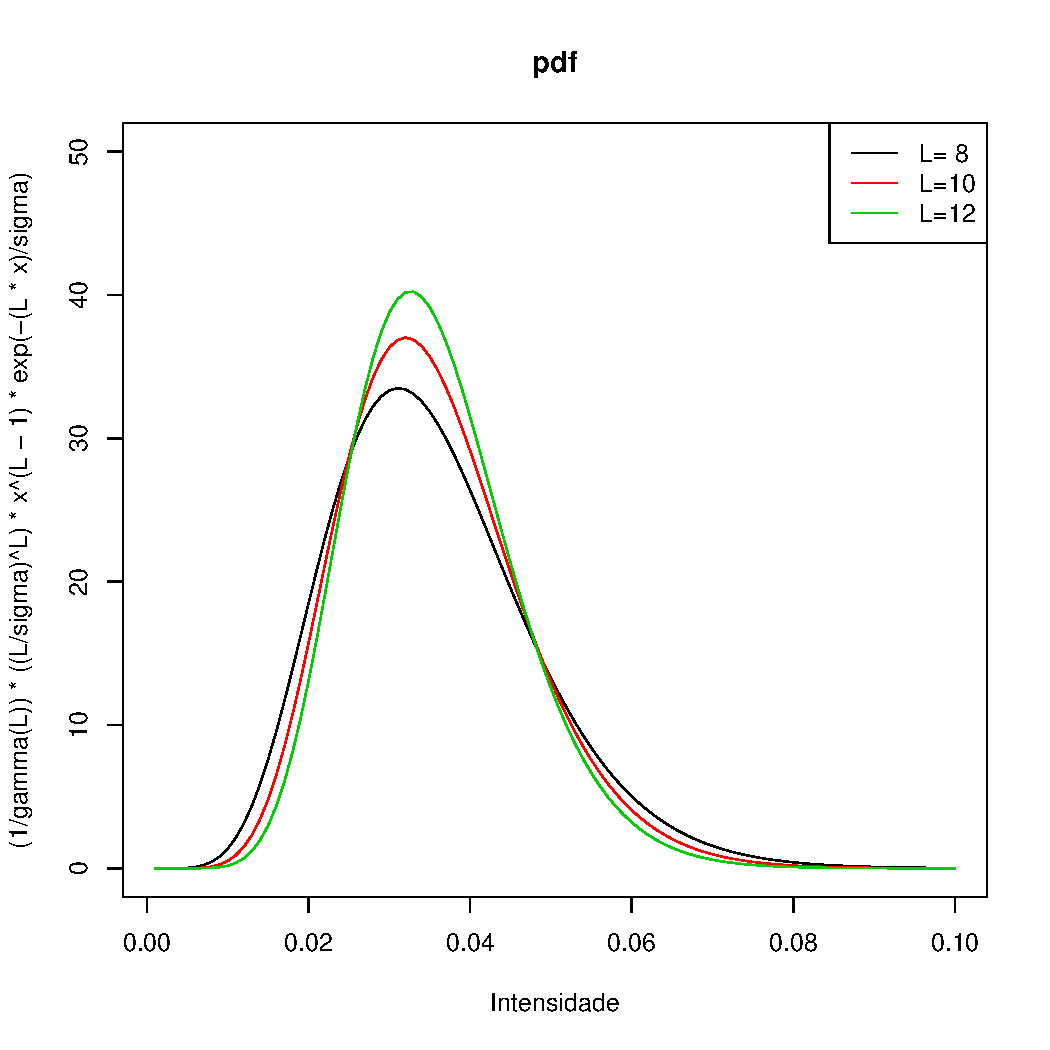
\includegraphics[width=4.0in]{fig_1_anfinsen_2009.pdf}
	\caption{Distribuição gamma da referência \cite{anfinsen2009} com parametros $\sigma=0.0356$ e $L=\{8,10,12\}$.}
\label{sec41fig1}
\end{figure}

\subsection{Estudo do artigo  \cite{freitas_frery_2005}}

As definições deste artigo são semelhantes as definições do artigo \cite{anfinsen2009} descrita na seção acima. 

\subsubsection{ Entendendo as densidades e seus gráficos}

Nesta seção o intuito é reproduzir e entender as distribuições que geraram as figuras (1), (2) e (3) do artigo \cite{freitas_frery_2005}. 

\begin{equation}\label{sec51eqn1}
\begin{array}{ccc}
	f_{X}(x)&=&\frac{r_{\alpha,\omega}}{2K_{\alpha}(\omega)}x^{\alpha-1}\exp\left(-\frac{\omega}{2}\left(\frac{1}{r_{\alpha,\omega}x}+ r_{\alpha,\omega}x\right)\right), \\
\end{array}
\end{equation}

onde $x>0$  e $r_{\alpha,\omega}=\frac{K_{\alpha+1}(\omega)}{K_{\alpha}(\omega)}$

Seja $K_{\nu}$ uma função de Bessel de terceiro tipo e com ordem $\nu$. Na figura (\ref{sec51fig1}) é mostrado os gráficos das funções para diferentes valores de $\nu=1,2,3,4,5,10$ e $\nu=20$. 
\begin{figure}[!htb]
\centering
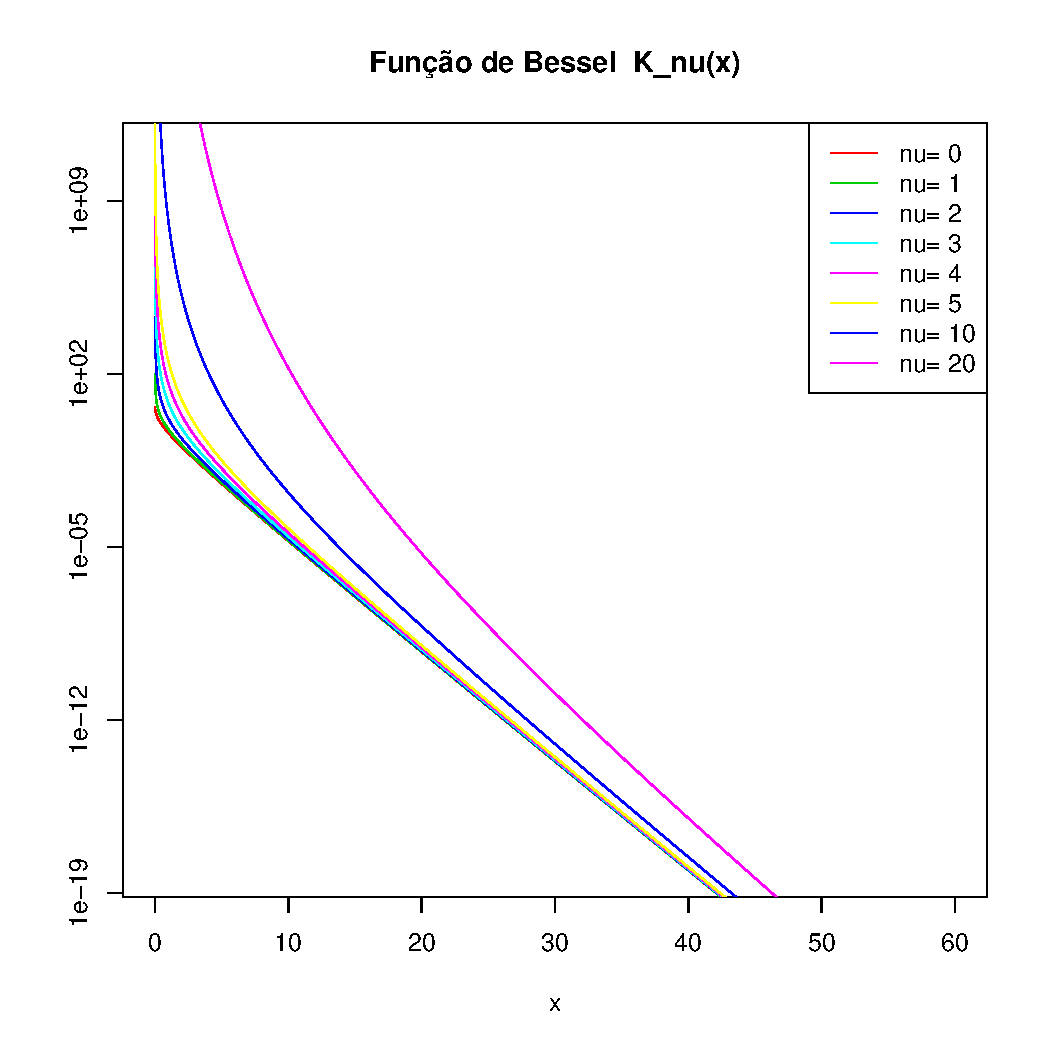
\includegraphics[width=4.0in]{fun_bessel_nu.pdf}
	\caption{Gráficos da referência \cite{freitas_frery_2005} para as funções de Bessel de terceiro tipo para diferentes $\nu$.}
\label{sec51fig1}
\end{figure}

A figura (\ref{sec51fig2}) mostra os gráficos da equação (\ref{sec51eqn1}) para $\omega=1$ e diferentes valores de $\alpha\in(1.1,3,10,20)$. 

\begin{figure}[!htb]
\centering
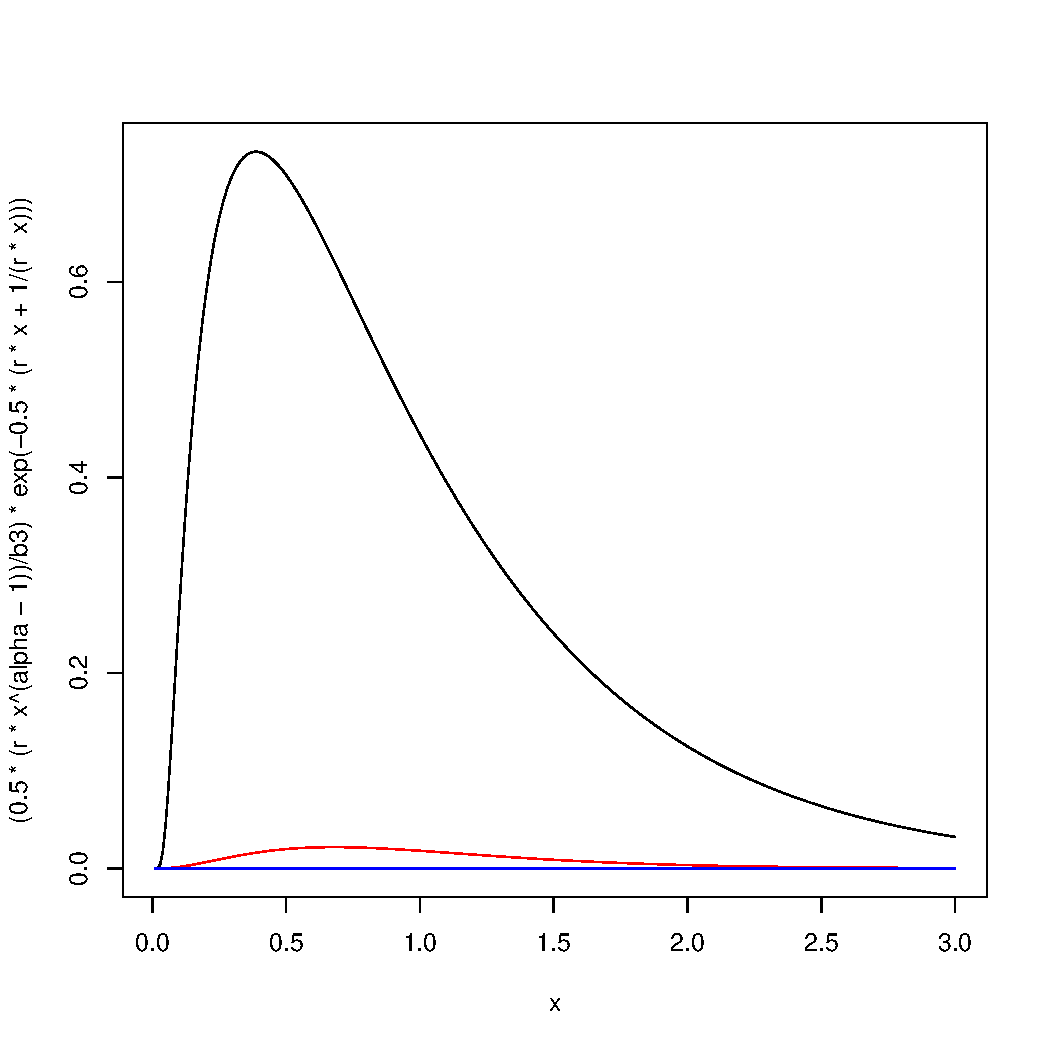
\includegraphics[width=4.0in]{fig1_freitas_frery_2005.pdf}
	\caption{Gráficos da referência \cite{freitas_frery_2005} para as equações (\ref{sec51eqn1}) para $\omega=1$ e $\alpha\in(1.1,3,10,20)$.}
\label{sec51fig2}
\end{figure}

A figura (\ref{sec51fig3}) mostra os gráficos da equação (\ref{sec51eqn1}) para $\alpha=1$ e diferentes valores de $\omega\in(1,2,10,30)$. 

\begin{figure}[!htb]
\centering
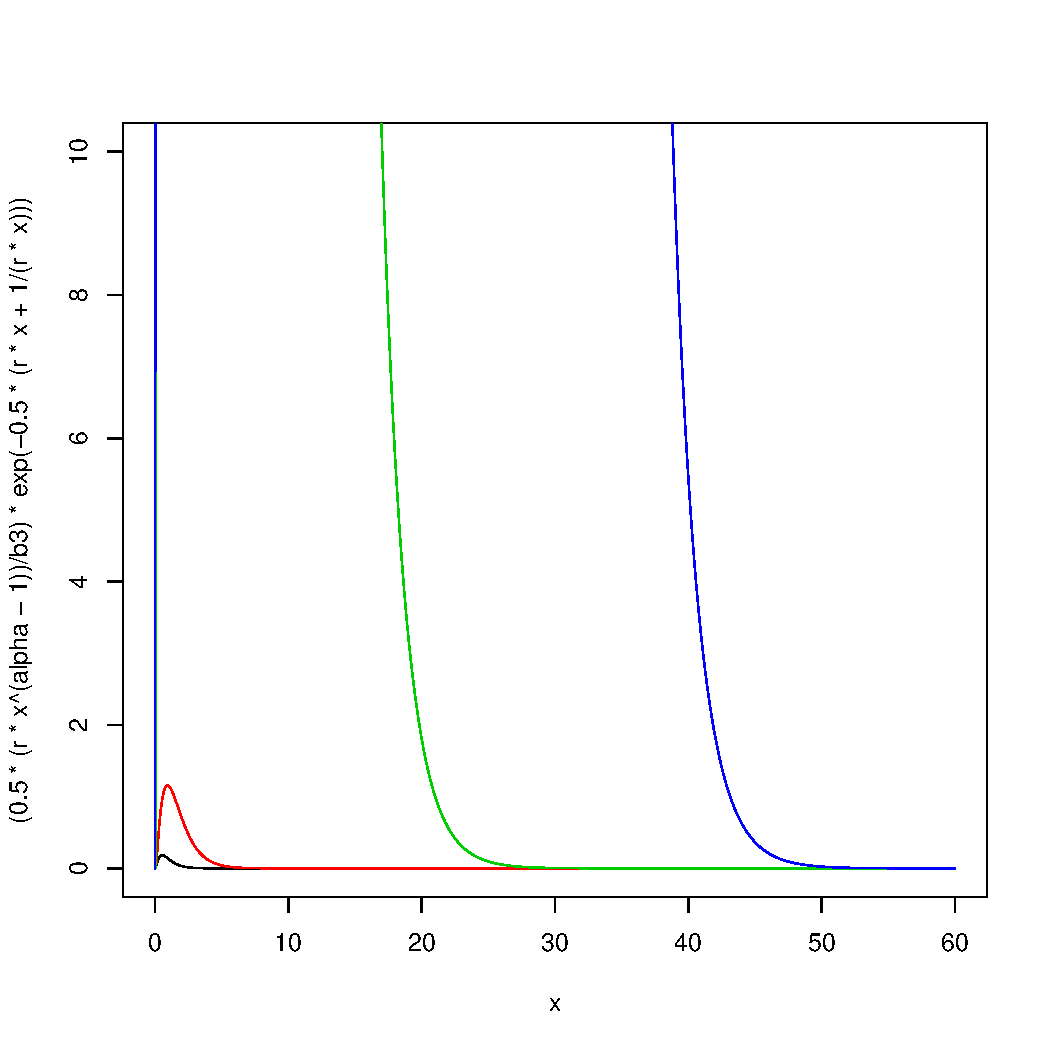
\includegraphics[width=4.0in]{fig2_freitas_frery_2005.pdf}
	\caption{Gráficos da referência \cite{freitas_frery_2005} para as equações (\ref{sec51eqn1}) para $\alpha=1$ e $\omega\in(1,2,10,30)$.}
\label{sec51fig3}
\end{figure}

	
As figuras (\ref{sec51fig2}) e (\ref{sec51fig3}) deste estudo deveriam estar equivalentes as figuras (1) e (2) do artigo \cite{freitas_frery_2005}, porém mostraram diferenças consideráveis nas magnitudes das funções. 

Para gerar as figuras (\ref{sec51fig1}), (\ref{sec51fig2}) e (\ref{sec51fig3}) usei a função de Bessel (besselk) programada no pacote R.

{\bf obs 2} - Programa {\it probesselfreitasfrery2005.r} armazenado no meu computador pessoal.

{\bf obs 3} - Programa {\it profig1freitasfrery2005.r} armazenado no meu computador pessoal.

{\bf obs 4} - Programa {\it profig2freitasfrery2005.r} armazenado no meu computador pessoal.

A densidade que caracteriza a distribuição gamma com média unitária

\begin{equation}\label{sec51eqn2}
\begin{array}{ccc}
	f_{X}(x)&=&\frac{\alpha^{\alpha}x^{\alpha-1}}{\Gamma(\alpha)}\exp\left(-\alpha x\right), \\
\end{array}
\end{equation}

onde $\alpha$,$x>0$, cujos gráficos estão na figura (\ref{sec51fig4}).

\begin{figure}[!htb]
\centering
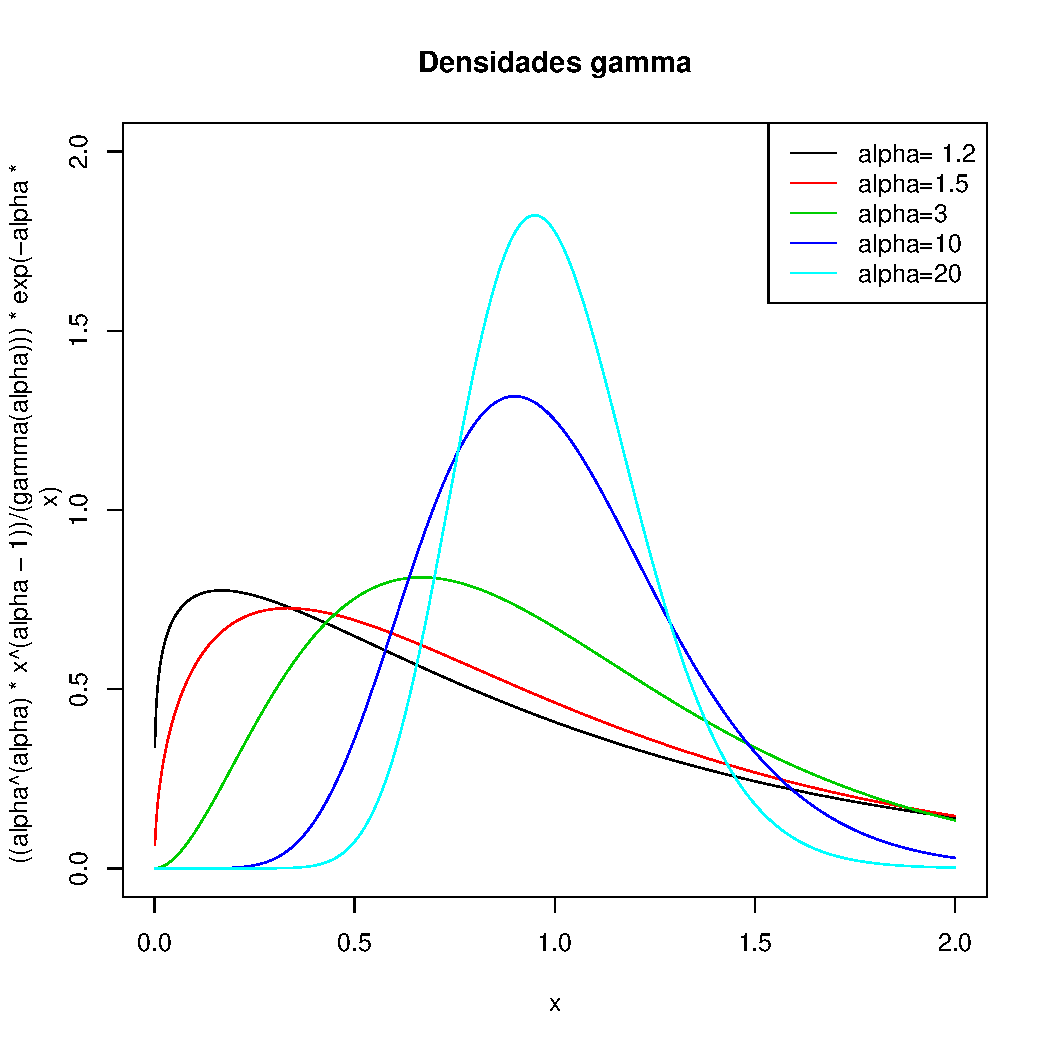
\includegraphics[width=4.0in]{fig3a_freitas_frery_2005.pdf}
	\caption{Densidades  gamma unitária (\ref{sec51eqn2}) para $\alpha > 0$ e $|\alpha|\in(1.2,1.5,3,10,20)$, referência \cite{freitas_frery_2005} .}
\label{sec51fig4}
\end{figure}


A densidade que caracteriza a distribuição gamma reciproca com média unitária

\begin{equation}\label{sec51eqn3}
\begin{array}{ccc}
	f_{X}(x)&=&\frac{x^{\alpha-1}}{(-\alpha-1)^{\alpha}\Gamma(-\alpha)}\exp\left(\frac{\alpha+1}{x}\right), \\
\end{array}
\end{equation}

onde $-\alpha$,$x>0$, cujos gráficos estão na figura (\ref{sec51fig5}).

\begin{figure}[!htb]
\centering
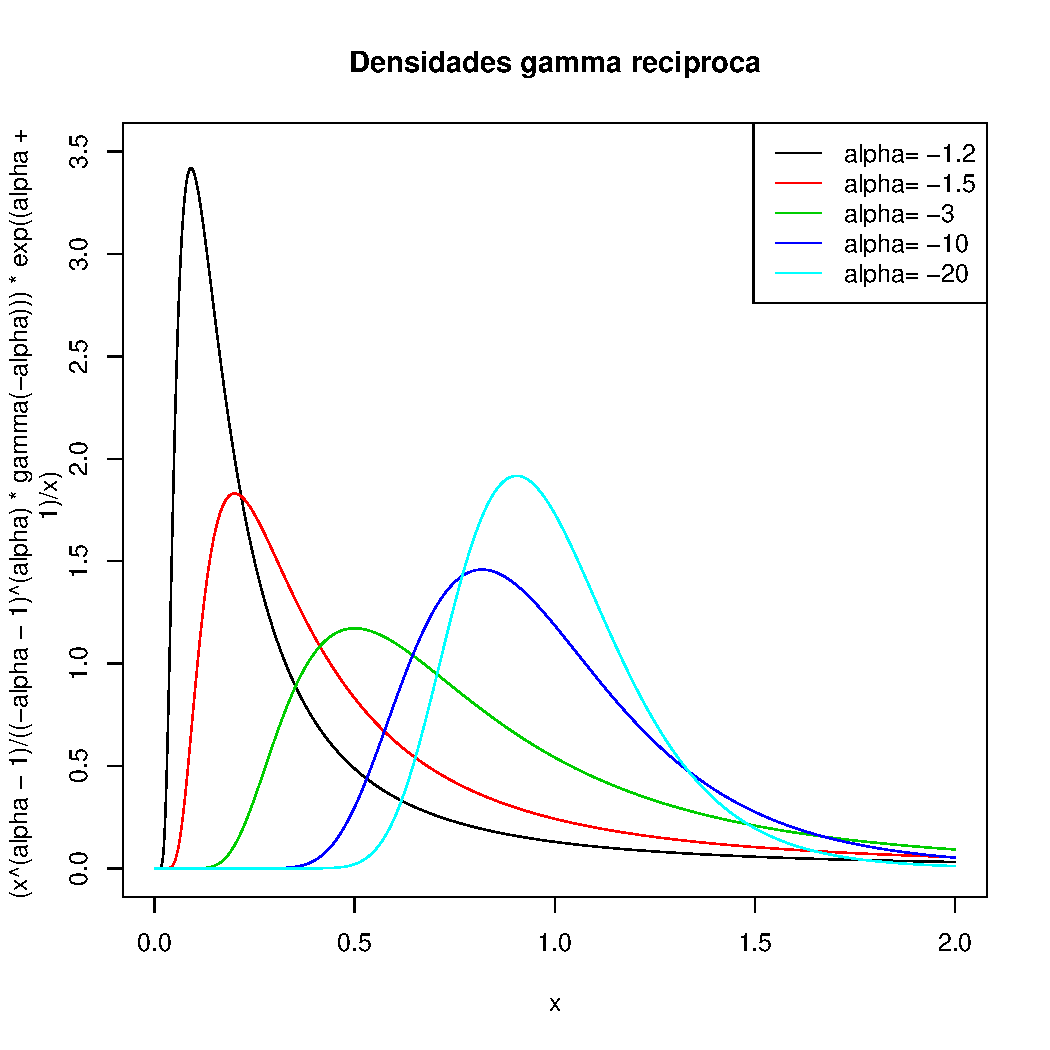
\includegraphics[width=4.0in]{fig3b_freitas_frery_2005.pdf}
	\caption{Densidades gamma unitária reciproca (\ref{sec51eqn3}) para $\alpha < 0$ e $|\alpha|\in(1.2,1.5,3,10,20)$, referência \cite{freitas_frery_2005} .}
\label{sec51fig5}
\end{figure}

{\bf obs 5} - Programa {\it profig3afreitasfrery2005.r} armazenado no meu computador pessoal.

{\bf obs 6} - Programa {\it profig3bfreitasfrery2005.r} armazenado no meu computador pessoal.

\subsection{Estudo do artigo  \cite{frery_muller_1997}}

No artigo é apresentado uma nova classe de distribuíções ${\it g}$ surgindo do modelo multiplicativo e um caso especial chamado {\it $g^{0}$} o qual se mostrou hábil para modelar  {\it extremely heterogeneus clutter}.


\subsubsection{O modelo multiplicativo e o ruído {\it speckle}}

Os ruídos {\it speckle} são associados a cenas "coerentes iluminadas" tais como as obtidas por microondas, laser, ultrasonografia, etc. É um tipo de ruído que apareçe devido a fenomênos de interferência entre o sinal incidente e o sinal refletido. Este tipo de ruído pode tornar a tarefa de interpretar a imagem tanto visual como automática difícil. 

O modelo multiplicativo é uma ferramenta usada para explicar o comportamento estatístico de dados obtidos com coerentes iluminação. Assumindo que a observação com estas imagens são o resultado do produto de duas independentes variáveis randômicas, uma $(X)$ modelando o retroespalhamento do terreno, e outra $(Y)$ modelando o ruído {\it speckle}. O primeiro é considerado real e positivo, enquanto o segundo pode ser complexo.

O valor observado é resultado da variável randômica definida como $Z=X\cdot Y$. Serão definidos os seguintes subescritos $C$, $I$, e $A$ para a referência a complexos, intensidade e amplitude respectivamente.

{\it Speckle} complexo tem distribuição normal bivariada com componentes distribuída identicamente independente tendo média $0$ e variância $\frac{1}{2}$. Assim, ${\bf Y}_{C}=(Y_{\mathbb{R}}, Y_{\mathbb{I}})\sim N2(0,\frac{1}{2})$ denota a distribuíção do par.

{\it Multilook intensity speackle} surge tomando a média sobre $n$ amostras independentes de $Y_{I}=\|Y_{C}\|^2$ na qual implica a distribuição gamma denotada por $Y_{I}\sim \Gamma(n,n)$ e caracterizado pela densidade mostrada na figura (\ref{sec61fig1})

\begin{equation}\label{sec61eqn1}
\begin{array}{ccc}
	f_{Y_{I}}(y)&=&\frac{n^{n}}{\Gamma(n)}y^{n-1}\exp\left(-ny\right),\quad y,n>0 \\
\end{array}
\end{equation}

\begin{figure}[!htb]
\centering
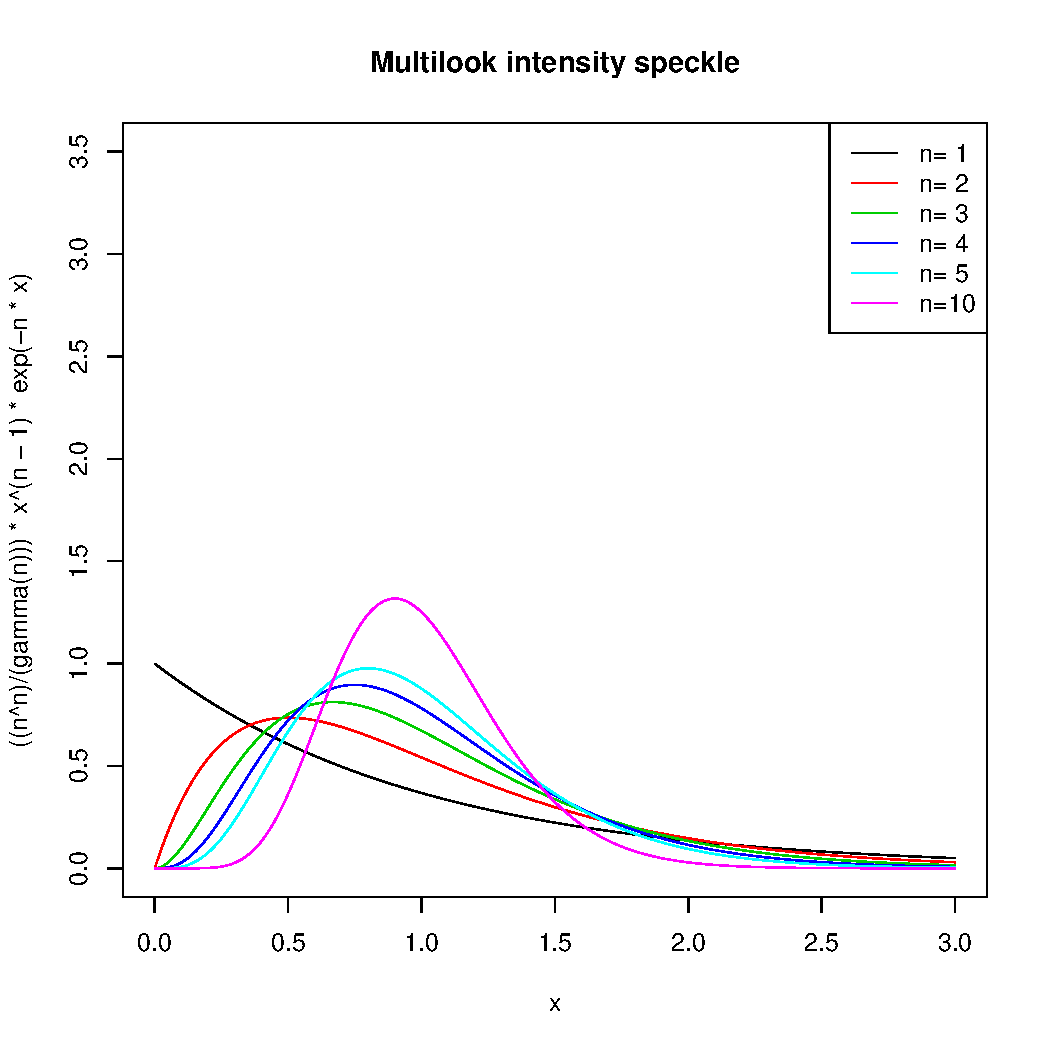
\includegraphics[width=4.0in]{fig_eq_fyi_frery_muller_1997.pdf}
	\caption{Multilook Intensity speckle  para $n\in(1,2,3,4,5,10)$.}
\label{sec61fig1}
\end{figure}

{\it Multilook amplitude speackle} surge tomando a raíz quadrada do {\it Multilook intensity speackle} e portanto a raíz quadrada da distribuíção gamma, denotado por $Y_{A}\sim \Gamma^{\frac{1}{2}}(n,n)$ e caracterizado pela densidade e mostrada na figura  (\ref{sec61fig2}).

\begin{equation}\label{sec61eqn2}
\begin{array}{ccc}
	f_{Y_{A}}(y)&=&\frac{2*n^{n}}{\Gamma(n)}y^{2*n-1}\exp\left(-ny^2\right),\quad y,n>0 \\
\end{array}
\end{equation}
\begin{figure}[!htb]
\centering
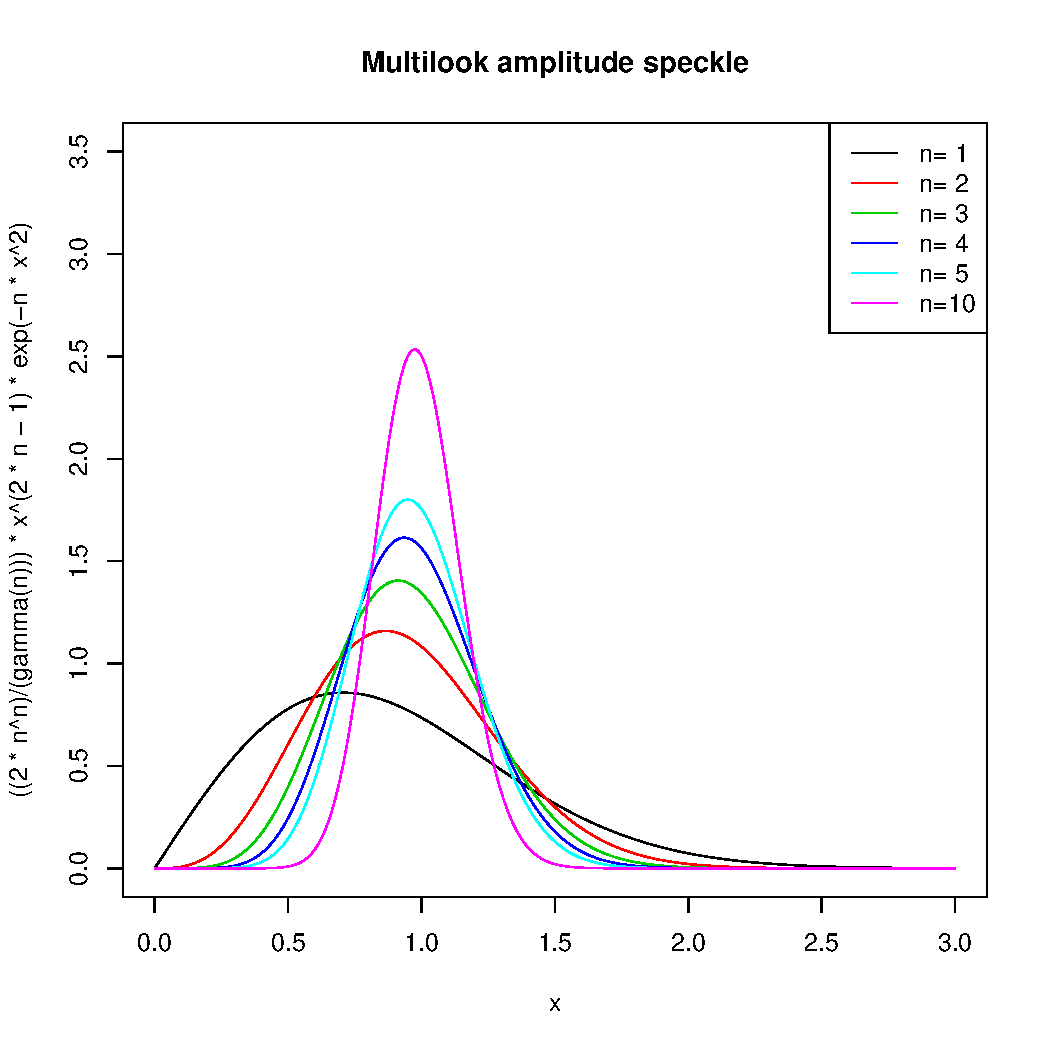
\includegraphics[width=4.0in]{fig_eq_fya_frery_muller_1997.pdf}
	\caption{Multilook Amplitude speckle  para $n\in(1,2,3,4,5,10)$.}
\label{sec61fig2}
\end{figure}
\subsubsection{Amplitude do retroespalhamento}

A amplitude do retroespalhamento obedeçe a raíz quadrada da lei gaussiana inversa generalizada, donotado aqui por ${\bf X}_{A}\sim N^{-\frac{1}{2}}(\alpha,\gamma,\lambda)$, sendo sua densidade dada por
\begin{equation}\label{sec62eqn1}
\begin{array}{ccc}
	f_{X_{A}}(x)&=&\frac{\left(\frac{\lambda}{\gamma}\right)^{\frac{\alpha}{2}}}{K_{\alpha}(2\sqrt{\lambda\gamma})}x^{2\alpha-1}\exp\left(-\frac{\gamma}{x^2}-\lambda x^2\right) \\
\end{array}
\end{equation}

Dois casos particulares desta distribuíção são de interesse na análise de dados $SAR$, a raíz quadrada de gamma e a reciproca da raíz quadrada da distribuição gamma. 

A raíz quadrada da distribuição gamma surge quando $\gamma \rightarrow 0$ enquanto $\alpha,\lambda>0$. Esta distribuição é denota aqui por $\Gamma^{\frac{1}{2}}(\alpha,\lambda)$ e caracterizada pela densidade 
\begin{equation}\label{sec62eqn2}
\begin{array}{ccc}
	f_{X_{A}}(x)&=&\frac{2\lambda^{\alpha}}{\Gamma(\alpha)}x^{2\alpha-1}exp(-\lambda x^2), \quad \alpha,\lambda, x>0. \\
\end{array}
\end{equation}
A reciproca da raíz quadrada da distribuição gamma surge quando $\lambda\rightarrow 0$ enquanto $-\alpha,\gamma>0$. Esta distribuição é denotada aqui por $\Gamma^{-\frac{1}{2}}(\alpha,\gamma) $ e caracterizada pela densidade
\begin{equation}\label{sec62eqn3}
\begin{array}{ccc}
	f_{X_{A}}(x)&=&\frac{2}{\gamma^{\alpha}\Gamma(-\alpha)}x^{2\alpha-1}exp(-\frac{-\gamma}{x^2}), \quad -\alpha,\lambda, x>0. \\
\end{array}
\end{equation}

\subsubsection{Retorno complexo}

Definindo uma distribuição geral $X_{A}$ como sendo $N^{-\frac{1}{2}}$ e dado um ruído complexo {\it speckle} é definido como $Y_{C}=(Y_{\mathbb{R}},Y_{\mathbb{I}})\sim N2(0,\frac{1}{2})$. assim é possível derivar uma distribuição marginal associada para o retorno complexo, o qual é dado por $Z_{C}=X_{A}\cdot Y_{C}=X_{
A}\cdot(Y_{\mathbb{R}},Y_{\mathbb{I}})$. A densidade que caracteriza a distribuição da parte real e da parte imaginária de $Z_{C}$, denotada por $Z_{\circ}$ e definida por
\begin{equation}\label{sec63eqn1}
\begin{array}{ccc}
	f_{Z_{\circ}}(x)&=&\frac{1}{K_{\alpha}(2\sqrt{\lambda\gamma})}\sqrt{\frac{\left(\frac{\lambda}{\gamma} \right)^{\alpha}}{\pi}}\left(\frac{\gamma+x^2}{\lambda} \right)^{\frac{\alpha-\frac{1}{2}}{2}}K_{\alpha-\frac{1}{2}}\left(2\sqrt{\lambda(\gamma+x^2)}\right), x\in\mathbb{R}. \\
\end{array}
\end{equation}

sendo o espaço do parâmetro dado por:
\begin{equation}\label{sec63eqn2}
	\left\{
\begin{array}{ccr}
	\gamma>0,&\lambda\geq 0&\mbox{se}\quad\alpha<0 \\
	\gamma>0,&\lambda > 0&\mbox{se}\quad\alpha=0 \\
	\gamma\geq0,&\lambda> 0&\mbox{se}\quad\alpha>0 \\
\end{array}
\right.
\end{equation}

Esta distribuição é denotada por $g_{C}(\alpha,\gamma,\lambda)$, o artigo mostra que a distribuição $g_{C}(\alpha,\gamma,\lambda)$ pode convergir em distribuição com condições estabelecidas no artigo para $K){C}(\alpha,\lambda)$(retroespalhamento heterogêneo) ou para $g_{C}^{0}$ (retroespalhamento extremamente heterogêneo).

A distribuição $K$ e $g^0$ podem ser representadas pelas equações respectivamente

\begin{equation}\label{sec63eqn3}
\begin{array}{ccc}
	f_{Z_{\circ}}(x)&=&\frac{2}{\Gamma(\alpha)}\sqrt{\frac{\lambda^{\alpha+\frac{1}{2}}}{\pi}} |x|^{\alpha-\frac{1}{2}}K_{\alpha-\frac{1}{2}}(2|x|\sqrt{\lambda}), \alpha,\lambda>0, x\in\mathbb{R}. \\
\end{array}
\end{equation}
\begin{equation}\label{sec63eqn4}
\begin{array}{ccc}
	f_{Z_{\circ}}(x)&=&\frac{\Gamma(\frac{1}{2}-\alpha)}{\sqrt{\pi}\gamma^{\alpha}\Gamma(-\alpha)}\left(x^2+\gamma\right)^{\alpha-\frac{1}{2}}, -\alpha,\lambda>0, x\in\mathbb{R}. \\
\end{array}
\end{equation}

\subsubsection{Retorno da amplitude}

A distribuição do retorno da distribuição surge de $Z_{A}=X_{A}Y_{A}$ onde $X_{A}\sim N^{-\frac{1}{2}}(\alpha,\gamma,\lambda)$  e $Y_{A}\sim\Gamma^{\frac{1}{2}}(n,n)$ é denotado por como $g_{A}(\alpha,\gamma,\lambda,n)$ é caracterizado pela densidade  

\begin{equation}\label{sec64eqn1}
\begin{array}{ccc}
	f_{Z_{\circ}}(x)&=&\frac{2n^n\left(\frac{\lambda}{\gamma}\right)^{\frac{\alpha}{2}}}{\Gamma(n)K_{\alpha}(2\sqrt{\lambda\gamma})}x^{2n-1}\left(\frac{\gamma+nx^2}{\lambda}\right)^{\frac{\alpha-n}{2}}K_{\alpha-n}(2\sqrt{\lambda(\gamma+nx^2)}), x\in\mathbb{R}. \\
\end{array}
\end{equation}
com o espaço de parametro (\ref{sec63eqn2}).

Onde $K_{A}$ e $g_{A}$  distribuição amplitude $K$ e a distribuição $g^0$ e podem ser representadas pelas equações abaixo respectivamente

\begin{equation}\label{sec64eqn2}
\begin{array}{ccc}
	f_{Z_{A}}(x)&=& \frac{4\lambda n x}{\Gamma(\alpha)\Gamma(n)}(\lambda n x^2)^{\frac{(\alpha+n)}{2}-1} K_{\alpha-n}(2x\sqrt{\lambda n}), \alpha,\lambda,n, x>0. \\
\end{array}
\end{equation}

\begin{equation}\label{sec64eqn3}
\begin{array}{ccc}
	f_{Z_{A}}(x)&=& \frac{2n^n\Gamma(n-\alpha)\gamma^{-\alpha}x^{2n-1}}{\Gamma(n)\Gamma(-\alpha)(\gamma+nx^2)^{n-\alpha}}, -\alpha,\gamma,n, x>0. \\
\end{array}
\end{equation}


As distribuições $g_A$ com a variação do parâmetros conforme o artigo estão representadas nas figuras (\ref{sec64fig1}) e (\ref{sec64fig2}).


\begin{figure}[!htb]
\centering
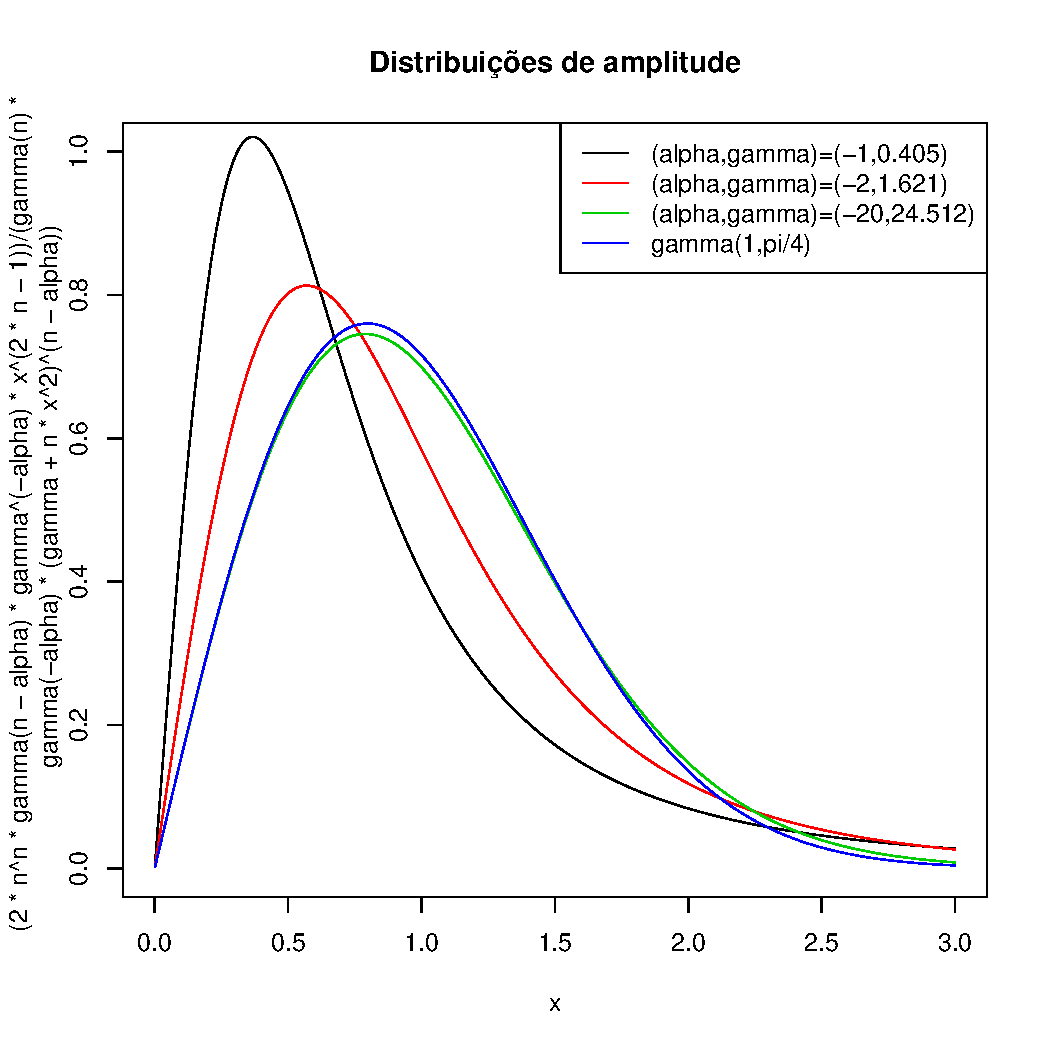
\includegraphics[width=4.0in]{fig_eq_ga_fig1_frery_muller_1997.pdf}
	\caption{Distribuições de amplitude.}
\label{sec64fig1}
\end{figure}

\begin{figure}[!htb]
\centering
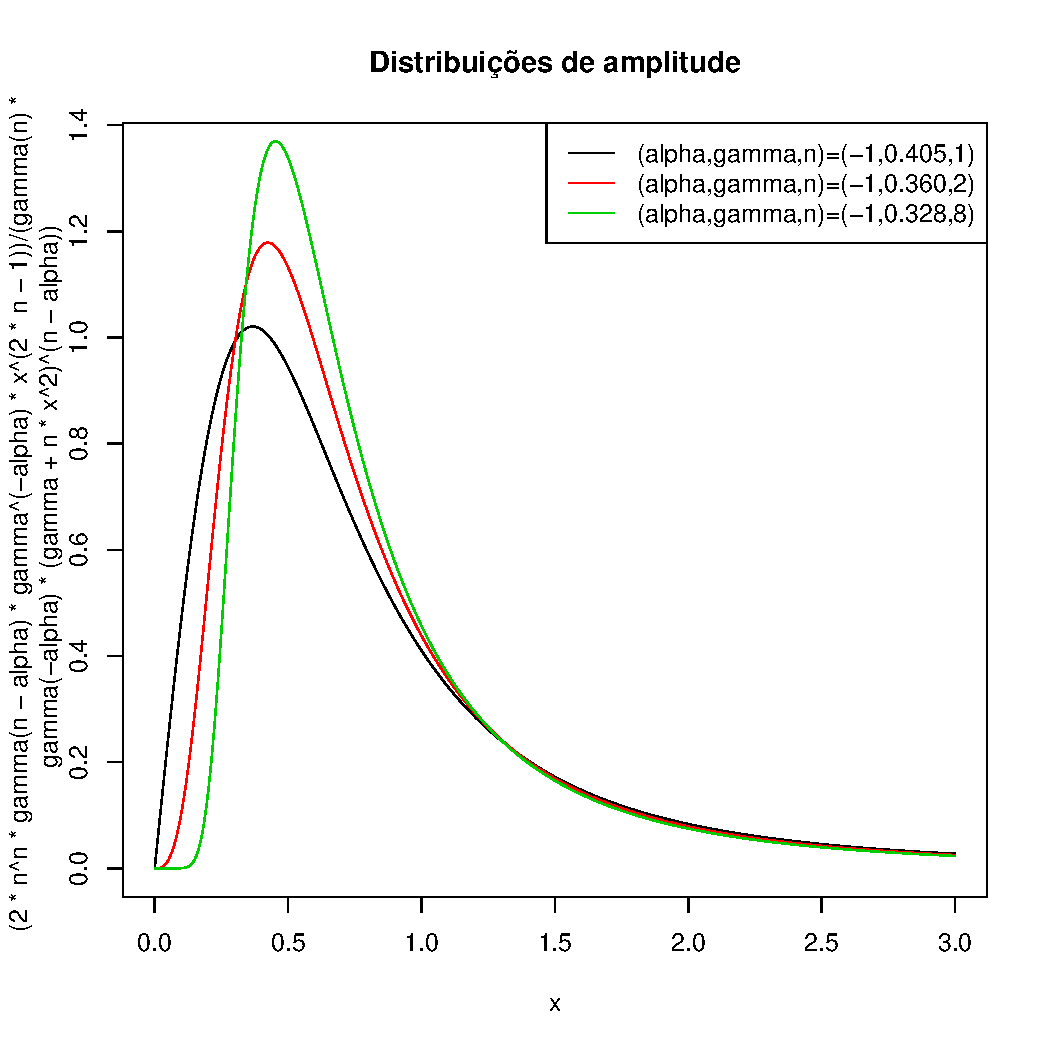
\includegraphics[width=4.0in]{fig_eq_ga_fig2_frery_muller_1997.pdf}
	\caption{Distribuições de amplitude.}
\label{sec64fig2}
\end{figure}

\subsubsection{Modelando áreas urbanas}

Quando estimamos os três parâmetros da distribuíção $g_A$ sobre áreas urbanas foi observado que o atrator e a solução global do sistema de equações estava  no subconjunto do espaço de parâmetros dado por ($\alpha<0,\gamma0,\lambda<10^{-6}$); 

\subsection{Estudo do artigo  \cite{frery_nascimento_2014}}.

\subsubsection{Distribuição complexa de Wishart}

\begin{equation}\label{sec71eqn1}
\begin{array}{ccc}
	f_{{\bf Z}}({\bf Z};{\bf \Sigma},L)&=&\frac{L^{pL}|{\bf Z}|^{L-p}}{|{\bf \Sigma}|^{L}\Gamma_d(L)} exp(-L\mathrm{tr}{({\bf \Sigma}^{-1}{\bf Z})}), \\
\end{array}
\end{equation}

A ideia é encontrar a derivada do logaritmo natural em relação ao número de {\it looks}, com esse intuito a ditribuição (\ref{sec71eqn1}) será reescrita
\begin{equation}\label{sec71eqn2}
\begin{array}{ccc}
	\ln{\left(f_{{\bf Z}}({\bf Z};{\bf \Sigma},L)\right)}&=&\ln{\left(\frac{L^{pL}|{\bf Z}|^{L-p}}{|{\bf \Sigma}|^{L}\Gamma_d(L)} \exp(-L\mathrm{tr}{({\bf \Sigma}^{-1}{\bf Z})})\right)}, \\
	\ln{\left(f_{{\bf Z}}({\bf Z};{\bf \Sigma},L)\right)}&=&\ln{\left(\frac{L^{pL}|{\bf Z}|^{L-p}}{|{\bf \Sigma}|^{L}\Gamma_d(L)}\right)}\ln{\left( exp(-L\mathrm{tr}{({\bf \Sigma}^{-1}{\bf Z})})\right)}, \\
	\ln{\left(f_{{\bf Z}}({\bf Z};{\bf \Sigma},L)\right)}&=&\ln{\left(L^{pL}|{\bf Z}|^{L-p}\right)} - \ln{\left(|{\bf \Sigma}|^{L}\Gamma_d(L)\right)}-L\mathrm{tr}{({\bf \Sigma}^{-1}{\bf Z})}, \\
	\ln{\left(f_{{\bf Z}}({\bf Z};{\bf \Sigma},L)\right)}&=&\ln{\left(L^{pL}\right)}+\ln{\left( |{\bf Z}|^{L-p}\right)} - \ln{\left(|{\bf \Sigma}|^{L}\right)}-\ln{\left(\Gamma_d(L)\right)}-L\mathrm{tr}{({\bf \Sigma}^{-1}{\bf Z})}, \\
	\ln{\left(f_{{\bf Z}}({\bf Z};{\bf \Sigma},L)\right)}&=&pL\ln{\left(L\right)}+(L-p)\ln{\left( |{\bf Z}|\right)} - L\ln{\left(|{\bf \Sigma}|\right)}-\ln{\left(\Gamma_d(L)\right)}-L\mathrm{tr}{({\bf \Sigma}^{-1}{\bf Z})}, \\
	\ln{\left(f_{{\bf Z}}({\bf Z};{\bf \Sigma},L)\right)}&=&pL\ln{\left(L\right)}+L\ln{\left( |{\bf Z}|\right)}-p\ln{\left( |{\bf Z}|\right)}- L\ln{\left(|{\bf \Sigma}|\right)}-\ln{\left(\Gamma_d(L)\right)}-L\mathrm{tr}{({\bf \Sigma}^{-1}{\bf Z})}, \\
\end{array}
\end{equation}


Derivando com relação ao número de {\it looks} $L$, teremos

\begin{equation}\label{sec71eqn3}
\begin{array}{ccc}
	\frac{\partial}{\partial L}\left(\ln{\left(f_{{\bf Z}}({\bf Z};{\bf \Sigma},L)\right)}\right)&=&\frac{\partial}{\partial L}\left(pL\ln{\left(L\right)}+L\ln{\left( |{\bf Z}|\right)}-p\ln{\left( |{\bf Z}|\right)} - L \ln{\left(|{\bf \Sigma}|\right)}-\ln{\left(\Gamma_d(L)\right)}-L\mathrm{tr}{({\bf \Sigma}^{-1}{\bf Z})}\right), \\
	\frac{\partial}{\partial L}\left(\ln{\left(f_{{\bf Z}}({\bf Z};{\bf \Sigma},L)\right)}\right)&=&\left(p\ln{\left(L\right)}+p\right)+\ln{\left( |{\bf Z}|\right)} - \ln{\left(|{\bf \Sigma}|\right)}-\frac{\partial}{\partial L}\ln{\left(\Gamma_d(L)\right)}-\mathrm{tr}{({\bf \Sigma}^{-1}{\bf Z})}, \\
	\frac{\partial}{\partial L}\left(\ln{\left(f_{{\bf Z}}({\bf Z};{\bf \Sigma},L)\right)}\right)&=&p\left(\ln{\left(L\right)}+1\right)+\ln{\left(\frac{|{\bf Z}|}{|\bf \Sigma|}\right)}-\frac{\Gamma^{\prime}_d(L)}{\Gamma_d(L)}-\mathrm{tr}{({\bf \Sigma}^{-1}{\bf Z})}. \\
\end{array}
\end{equation}

Sendo $n$ tomado arbitrariamente entre o $L$ {\it looks} temos a seguinte equação
\begin{equation}\label{sec71eqn4}
\begin{array}{ccc}
	\frac{\partial}{\partial n}\left(\ln{\left(f_{{\bf Z}}({\bf Z};{\bf \Sigma},n)\right)}\right)&=&p\left(\ln{\left(n\right)}+1\right)+\ln{\left(\frac{|{\bf Z}|}{|\bf \Sigma|}\right)}-\frac{\Gamma^{\prime}_d(n)}{\Gamma_d(n)}-\mathrm{tr}{({\bf \Sigma}^{-1}{\bf Z})}. \\
\end{array}
\end{equation}

\bibliographystyle{unsrt}
\bibliography{../bibliografia} 
\end{document}
